\documentclass[11pt,twocolumn]{article}
\usepackage[margin=0.8in]{geometry}                % See geometry.pdf to learn the layout options. There are lots.
\geometry{letterpaper}                   % ... or a4paper or a5paper or ... 
%\geometry{landscape}                % Activate for for rotated page geometry
%\usepackage[parfill]{parskip}    % Activate to begin paragraphs with an empty line rather than an indent
\usepackage[breaklinks=true, colorlinks=true, linkcolor=red, urlcolor=blue, citecolor=black]{hyperref}
\urlstyle{rm}
\usepackage{amsmath}
\usepackage{mathptmx}
\usepackage{graphicx}
\usepackage{amssymb}
\usepackage{epstopdf}
\usepackage{color}
\usepackage{sidecap}
\usepackage{authblk}
\usepackage{booktabs}
\usepackage[font=small,labelfont=bf]{caption}
\DeclareGraphicsRule{.tif}{png}{.png}{`convert #1 `dirname #1`/`basename #1 .tif`.png}
\usepackage{enumitem}
\setlist[itemize]{noitemsep}
\setlist[enumerate]{noitemsep}

\def\bfr{\bf\color{red}}
\def\geohub{{\tt geohub}}
\def\Count{count}
\def\ntracts{39}
\def\nprof{9}
\def\nvol{30}
\def\resp{respectively}

\title{\bf
	Results of the 2021 Greater Hollywood Volunteer Homeless Count
	}
\author[1,2,3,$\dagger$]{Louis Abramson, PhD}%,$\ddagger$
\author[4]{Brian Kohan}%,$\ddagger$
\author[1,5]{Jackie Vorhauer}%,$\ddagger$
\author[1,6]{Heather Carmichael}%,$\ddagger$
\author[1,7]{Helen Eigenberg}%,$\ddagger$
\author[1,8]{Stephen Fiechter}%,$\ddagger$
\author[1]{David Gordon}%,$\ddagger$
\author[1,9]{Emily Uyeda Kantrim}%,$\ddagger$
\author[1,9]{Arnali Ray}%,$\ddagger$
\author[1,5]{Douglas Walker}%,$\ddagger$
\author[1]{Kerry Morrison}%,$\ddagger$
\affil[1]{\it \small Hollywood 4WRD Homelessness Coalition, 6255 Sunset Blvd, Ste 150, Los Angeles, CA 90028}
\affil[2]{\it Central Hollywood Neighborhood Council, PO Box 93907, Los Angeles, CA 90093}
\affil[3]{\it Carnegie Observatories, 813 Santa Barbara St, Pasadena, CA 91101}
\affil[4]{\it SELAH Neighborhood Homeless Coalition, \bf address}
\affil[5]{\it The Center at Blessed Sacrament, 6636 Selma Ave, Los Angeles, CA 90028}
\affil[6]{\it My Friend's Place, 5850 Hollywood Blvd, Los Angeles, CA 90028}
\affil[7]{\it Hang Out Do Good, \bf address}
\affil[8]{\it People Assisting The Homeless, 340 N Madison Ave, Los Angeles, CA 90004}
\affil[9]{\it Mid City West Community Council, 644 N Fuller Ave, PMB 7059, Los Angeles, CA 90036}
\affil[$\dagger$]{Corresponding author; \href{mailto:labramson.chnc@gmail.com}{labramson.chnc@gmail.com}}

\date{\today}                                           % Activate to display a given date or no date

\begin{document}
\maketitle

\begin{abstract}

A February 25, 2021 census of Hollywood and East Hollywood suggests that 
unsheltered homelessness has fallen in those communities by $11\%$ and $15\%$, \resp, compared to 
the 2020 LAHSA Point-In-Time (PIT) count. A 30\% drop in individuals seen on the street drives this 
change, reducing the number of identified persons and dwellings in 
about a third of census tracts. Unsheltered living is thus likely to have declined quantitatively even if the 
average occupancy of, e.g., tents is updated. However, 13\% of tracts
saw at least a doubling in street dwellings. This trend may contribute to qualitative perceptions that the 
state of homelessness has worsened over the past year, which---given COVID-related reductions in 
health, hygiene, and social support services---are also likely to be accurate.
Coordinated Entry System data will reveal whether homelessness has declined in toto or if 
government initiatives reduced only the portion of people living unsheltered in Greater Hollywood.

\end{abstract}

\section{Introduction}
\label{sec:intro}

The Los Angeles Homelessness Services Authority (LAHSA) typically conducts a Point In Time (PIT) 
census of the unhoused population of Los Angeles County annually. These data inform programmatic
funding levels, educate residents, undergird local and state legislative efforts, and shape the day-to-day 
practices of thousands of professional and volunteer service providers. As the official assessment of the 
scope of one of the most pressing humanitarian issues of our time, the LAHSA Count is invaluable.
However, due to disruptions from COVID-19, LAHSA decided to cancel the unsheltered portion
of the 2021 PIT count. As roughly 70\% of LA's unhoused residents are unsheltered, this move ensures
data on homelessness immediately following one year of unprecedented economic disruptions and
government interventions will be substantially incomplete.

Greater Hollywood is an epicenter of LA's homelessness crisis. According to the official 2020 
Count, the Hollywood and East Hollywood Communities were home to 2203 unhoused residents,
1714 of whom (78\%) were unsheltered. This figure corresponds to roughly 5\% of LA's homeless 
population concentrated in an area with only 2.5\% ({\bfr CITE}) of its total population. In some 
regions in those communities, 1-in-30 residents are unhoused compared to 1-in-100 citywide.

\begin{figure*}
	\centering
	\includegraphics[width=0.9\linewidth]{countMap}
	\caption{The 2021 volunteer \Count\ covered Greater Hollywood, comprising the 
			officially recognized LAHSA Hollywood and East Hollywood Continua
			of Care. The former stretches from Laurel Canyon Blvd to Western Ave,
			the latter from Western to Hoover Ave. Hollywood is bounded to the north
			and south respectively by Franklin	and Melrose Aves, with East Hollywood
			bounded by Hollywood Blvd and Beverly Ave. Hollywood comprises
			21 census tracts; East Hollywood 18.}
	\label{fig:map}	
\end{figure*}

While the above statistics are tragic, Hollywood is also marked by increasingly formal coalitions of 
service providers, business leaders, residents, and quasi-governmental entities dedicated to humanely 
ending the homelessness crisis. Each of these stakeholders relies on the annual PIT count: lay residents need
to be educated as to the size of the challenge; funders need to understand how many people require services;
legislators need to know how many people are dwelling where. For these reasons, and given the 
capacity of the above organizations and individuals, the Hollywood community decided to proceed with 
an unsponsored 2021 grassroots PIT \Count.

This document describes the methodology and findings of that \Count, which took place on Thursday, 
February 25, 2021. Section \ref{sec:procedure} describes data acquisition, analysis, and volunteer
training protocols. Section \ref{sec:results} present estimates of the unsheltered 
populations in the Hollywood and East Hollywood CoCs and contextualizes those findings in terms of 
previous LAHSA results. Section \ref{sec:systematics} describes factors that would
modulate them up or down. Section \ref{sec:summary} summarizes. Additional information
can be found in the Appendix, including a table of tract-level results in each of the survey's 39 US 
Census tracts.

\section{Methodology}
\label{sec:procedure}

Our \Count\ took place on 25 February 2021, with the majority of census tracts surveyed beginning
at 7.00 PM. This timing corresponds to one month later and four hours earlier than the official event 
would have occurred. Beyond those choices, our program adhered as closely as possible to the official 
LAHSA 2020 PIT data collection and analysis protocols. Ancillary data from regularly monitored 
census tracts suggests that the date offset is unlikely to substantially erode comparability between 
this and past datasets. Limited daytime recounts also suggest that time-of-day effects are sub-dominant.

The \Count\ was based out of The Center at Blessed Sacrament (``The Center''), a major service 
provider in Hollywood, at 6636 Selma Ave. All volunteer teams launched from and returned to this 
location as they would in previous years to a LAHSA community count hub. The major difference 
was that training was performed remotely as a COVID precaution and volunteer counters never left 
their vehicles.

\subsection{Data Acquisition}
\label{sec:acquisition}

The \Count\ covered the \ntracts\ US Census tracts constituting the LAHSA-defined Hollywood 
and East Hollywood Communities (21 and 18 tracts, \resp). Our \Count\ did not recognize census 
tract ``splits'' or sub-tracts---e.g., ``1905.10a''---which sets a coarser resolution floor to our results 
compared to past PIT results. That choice also slightly modifies of the definition of both communities:
Hollywood includes all of tract 1905.10 as opposed to only the ``a'' sub-tract, and East Hollywood
includes all of 1913.01 instead of just the ``b'' sub-tract. Such modifications have an insignificant impact 
on community-level results---since 2016, 1905.10b has never been seen to host more than 7 
unsheltered people; 1913.01a never more than 15. Sections \ref{sec:results} and \ref{sec:discussion} 
discuss community-level results with tract-level tallies provided in the Appendix. Results for Greater 
Hollywood are not directly comparable to any official service geography but are available upon request. 
Figure \ref{fig:map} shows the \Count\ footprint.

All tracts were vetted by professionals from The Center prior to assignment. Tracts deemed 
especially challenging---due, e.g., to their proximity to freeway onramps and peripheries---were 
reserved for professional counting teams. Vetting produced \nprof\ such tracts, which were surveyed 
by outreach personnel from The Center and Covenant House---another local provider---circa 3:00 PM
on 25 February. The remaining \nvol\ tracts were divided among the volunteer vehicle-based teams 
and surveyed beginning at 7.00 PM. Importantly, with the exception of one tract in East Hollywood, 
teams were restricted to one or the other community, making the community-level results nearly
independent. Cross-comparisons therefore serve as data quality indicators (Section \ref{sec:discussion}). 
Table \ref{tbl:tractStats} records which tract was counted by which kind of team. 

Thirty-two volunteer vehicle-based teams participated in the \Count\ itself, which was limited to 
existing COVID ``pods'' of two to three people to ensure that the possibility of transmission minimized. 
Singlet volunteers were admitted but remained on-site to assist with traffic control and material distribution. 
All participants wore personal protective equipment and maintained social distancing when appropriate.

Counting followed 2020 LAHSA PIT protocols to the greatest extent possible. Each vehicle-based 
volunteer team comprised at least a Driver and a Counter and was assigned two tracts to count. 
Three-person teams also included a Navigator. In such teams, the Navigator directed the Driver while 
the Counter tallied unhoused individuals/dwellings. In two-person teams, the Counter doubled as 
the Navigator. Training emphasized techniques aimed at reducing the Counters' cognitive loads and 
so minimize counting errors. These included driving slowly using hazard lights and covering interior 
streets in a serpentine pattern before circling the tract border. Teams were instructed to count both 
sides of interior streets but only interior sides of border streets. Teams were also instructed to watch
the official training video from the 2020 PIT count in addition to receiving the training from our
team.

Upon arriving at The Center, organizers gave each team a clipboard with:
\begin{itemize}
	\item tract maps (2$\times$);
	\item tally sheets (2$\times$);
	\item a 1-page training summary with a contact number for in-field issues.
\end{itemize}
Examples of each of the above documents are included in the Appendix. The latter was used 
once to alert site volunteers to the possibility of an unaccompanied minor.

The tally sheets---the data acquisition tool---contained separate columns for each of the nine 
categories of unhoused individuals or dwellings recognized in the 2020 LAHSA PIT count: 
\begin{enumerate}
	\item adults (ages $\geq$25);
	\item transition age youths (``TAY,'' 18--24);
	\item unaccompanied minors;
	\item families (at least one adult with at least one minor); 
	\item cars;
	\item vans;
	\item RVs;
	\item tents;
	\item makeshift structures.
\end{enumerate}
The dwelling classes---Items 5--9---are treated differently than the individual classes in the analysis,
and are hereafter referred to by their acronym, ``CVRTM,'' when appropriate. 

All teams were deployed to their tracts by roughly 7:30 PM and returned by 9:55 PM.

Upon returning, organizers approached each team with a tablet computer or smartphone. Counters 
verbally read-off their results for each category as organizers entered them into a google 
form/spreadsheet. The organizer read back the results for confirmation before recovering all 
materials---including hand-written tallies---from the volunteers. Volunteer email addresses 
were also retained for follow-up. 

Once all materials were collected, the organizers convened to cross-check the electronic records
with the physical tally sheets and identify any uncounted areas. Any disagreement between electronic
and paper references was cross-checked and corrected to the paper tally.

Given the number of volunteers, every tract was counted by at least two volunteer teams, with four
tracts counted in triplicate. Such repeat measurements were designed to aid understanding of random 
counting errors (Sections \ref{sec:dupes}) but also served a data robustness purpose: one tally
could not be associated with a census tract and therefore had to be removed. 

All told, the data set comprises 37 pair-wise volunteer measurements---29 duplicates + 
4 triplicates (=8 additional pairs)---and 9 unique professional assessments.


\begin{table}[t!]
\caption{Tract-level Unsheltered Population Summary}
\resizebox{\linewidth}{!}{%
\begin{tabular}{cccccc}
\toprule
Tract & Community & Counter & Passes & Median Est. & 90\% CI \\ 
 & & & & [people] & [people] \\ \cmidrule{1-6}
1898.00 & Hollywood & Vol & 3 & 6 & 0--15 \\
1899.02 & Hollywood & Vol & 3 & 18 & 12--24 \\
1899.03 & Hollywood & Vol & 2 & 0 & 0--12 \\
1899.04 & Hollywood & Vol & 2 & 18 & 11--25 \\
1899.05 & Hollywood & Vol & 2 & 19 & 9--30 \\
1901.00 & Hollywood & Vol & 2 & 88 & 75--102 \\
1902.01 & Hollywood & Vol & 2 & 21 & 13--29 \\
1902.02 & Hollywood & Vol & 2 & 30 & 20--40 \\
1903.01 & Hollywood & Pro & 1 & 74 & 54--96 \\
1905.10 & Hollywood & Pro & 1 & 34 & 22--46 \\
1905.20 & E.~Hollywood & Vol & 2 & 12 & 6--18 \\
1907.00 & Hollywood & Vol & 2 & 110 & 93--127 \\
1908.01 & Hollywood & Vol & 2 & 63 & 50--76 \\
1908.02 & Hollywood & Pro & 1 & 71 & 54--90 \\
1909.01 & Hollywood & Pro & 1 & 55 & 39--71 \\
1909.02 & Hollywood & Vol & 3 & 6 & 0--17 \\
1910.00 & Hollywood & Pro & 1 & 169 & 140--201 \\
1911.10 & E.~Hollywood & Vol & 2 & 9 & 2--15 \\
1911.20 & E.~Hollywood & Pro & 1 & 66 & 48--85 \\
1912.01 & E.~Hollywood & Vol & 2 & 55 & 44--68 \\
1912.03 & E.~Hollywood & Vol & 2 & 26 & 14--38 \\
1912.04 & E.~Hollywood & Vol & 2 & 6 & 0--16 \\
1913.01 & E.~Hollywood & Vol & 2 & 31 & 22--42 \\
1913.02 & E.~Hollywood & Vol & 2 & 23 & 15--30 \\
1914.10 & E.~Hollywood & Vol & 2 & 20 & 13--28 \\
1914.20 & E.~Hollywood & Vol & 2 & 24 & 16--32 \\
1915.00 & E.~Hollywood & Vol & 2 & 29 & 21--38 \\
1916.10 & E.~Hollywood & Pro & 1 & 48 & 31--68 \\
1916.20 & E.~Hollywood & Pro & 1 & 17 & 6--30 \\
1917.10 & Hollywood & Vol & 2 & 21 & 14--29 \\
1917.20 & Hollywood & Vol & 3 & 21 & 12--31 \\
1918.10 & Hollywood & Vol & 2 & 24 & 14--34 \\
1918.20 & Hollywood & Vol & 2 & 16 & 10--23 \\
1919.01 & Hollywood & Vol & 2 & 60 & 49--72 \\
1925.10 & E.~Hollywood & Vol & 2 & 12 & 4--21 \\
1925.20 & E.~Hollywood & Vol & 1 & 14 & 1--28 \\
1926.10 & E.~Hollywood & Vol & 2 & 7 & 1--14 \\
1926.20 & E.~Hollywood & Vol & 2 & 18 & 9--26 \\
1927.00 & E.~Hollywood & Pro & 1 & 129 & 96--167
\\ \bottomrule
\end{tabular}
}
\caption*{Counter denotes volunteer vs.~professional team; passes denote number of
		independent counts per tract.}
\label{tbl:tractStats}
\end{table}

\subsubsection{Volunteer Training}
\label{sec:training}

Teams underwent mandatory, $\sim$30 minute Zoom-based training sessions before arriving 
for the \Count. Each participant was also required to watch the official 2020 LAHSA count training 
video and sign participation waivers.

The training covered the motivation for the \Count, an overview of the survey geography, team roles, 
and examples of the classes of unhoused individuals/dwellings. Except in the case of people standing 
next to tents---as describes in the 2020 LAHSA video---volunteers were instructed to count 
CVRTM and individuals separately and not to try to estimate how many people might live in or be 
associated with a specific dwelling. This ensured that results could be analyzed as a function of the 
CVRTM weights, which may change with future information (see Section \ref{sec:analysis}).

Volunteers were primed only with min/max estimates of tract-level individual+dwelling counts 
(``0--120'') and the likelihood of encountering unaccompanied minors or families (``very unlikely'')
or TAY (``in some tracts in Hollywood''). These statements were informed by the 2020 LAHSA PIT 
results. No other prior count-based information was established to minimize biases. The training 
presentation is available at: \url{https://drive.google.com/file/d/1xFrtU26yjPuiUv9KHZ3Uj2_sAoT1ClGo/view?usp=sharing}.

In sum, about 20\% of tracts in both communities were counted by professionals. The latter comprised
roughly 43\% of the total individuals and dwellings counted. Year-on-year trends are consistent between
volunteer- and professionally counted tracts. The largest increase was observed by volunteers, the largest
decrease by professionals; both tracts are located in E.~Hollywood.

\subsection{Data Analysis}
\label{sec:analysis}

The core component of the raw data was a $9\times73$ spreadsheet containing the
tract-level tallies for each unhoused individual/dwelling class. Repeat counts of the same
tract associated with the Hollywood or East Hollywood community, were averaged, and
unweighted where appropriate by the CVRTM mean occupancies. This process was repeated 
10,000 times randomly perturbing the counts and weights according to their respective 
uncertainties (see below). The result is a $9\times10000\times39$ array can then 
be split and summed to provide aggregate, tract, or category-level unsheltered
population estimates and uncertainties.

Our baseline result incorporates the 2020 SPA-4/CD13 estimates of the CVRTM weights provided
by LAHSA. These estimates underpin the latest LAHSA Community Summaries. We recognize 
that COVID-related activities may have changed these weights---e.g., via concerted tent distribution
efforts---since the last PIT count and analyze the impact of various CVRTM choices in 
Section \ref{sec:CVRTM}. However, reasonable modifications---including those based on updated
occupancy surveys---do not significantly affect our findings.

%While an estimate of the underlying population, uncertainties in each visual count and weight 
%must be accounted for to understand how confident one can be that that estimate corresponds to
%the truth. We accomplish this by using Monte Carlo integration to construct the full probability
%distribution functions (PDFs) for the number of unsheltered people of each class in each tract.

% {\it These results will
%correspond to the most likely values for the respective quantities in any geography.} However,
%three uncertainties---one small and two large---complicate the interpretation of those sums. 
%We discuss these in Section \ref{sec:discussion}, but account for them as best we can using 
%Monte Carlo techniques to construct the full underlying probability distribution functions (PDFs) 
%for each class in each tract.
%
%All results discussed below derive from 10,000 Monte Carlo realizations of Item (5), above.
%

\begin{figure}[t]
\centering
	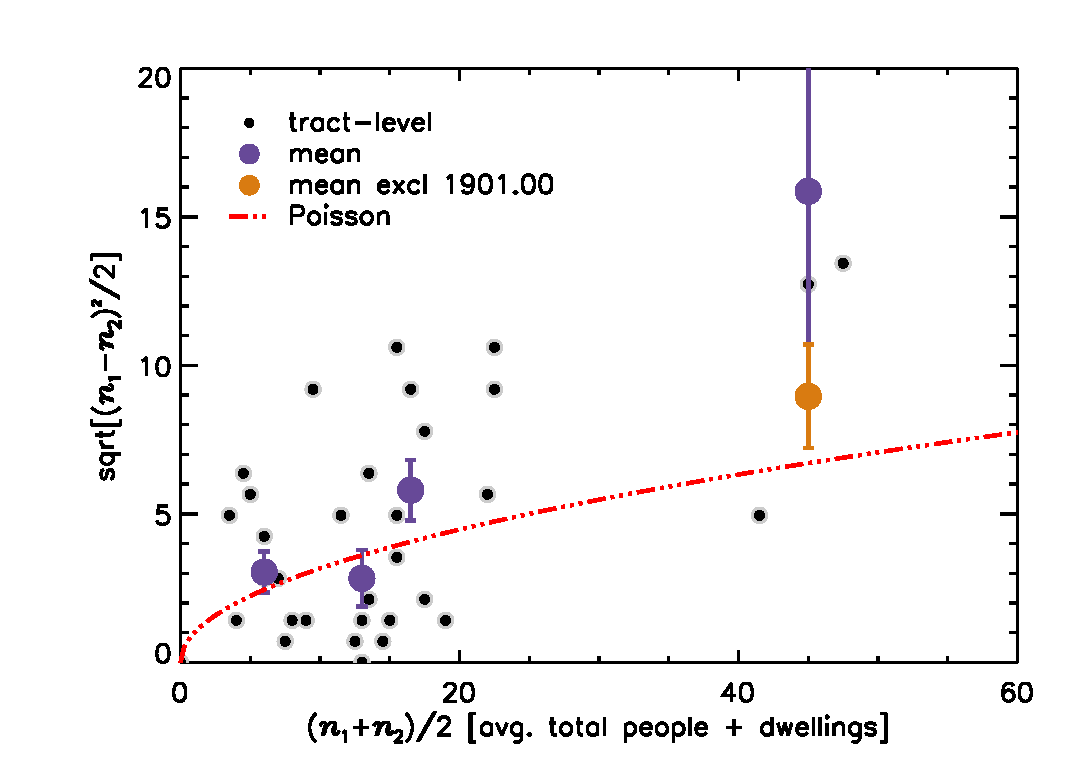
\includegraphics[width=\linewidth]{intDupeChar}\\
	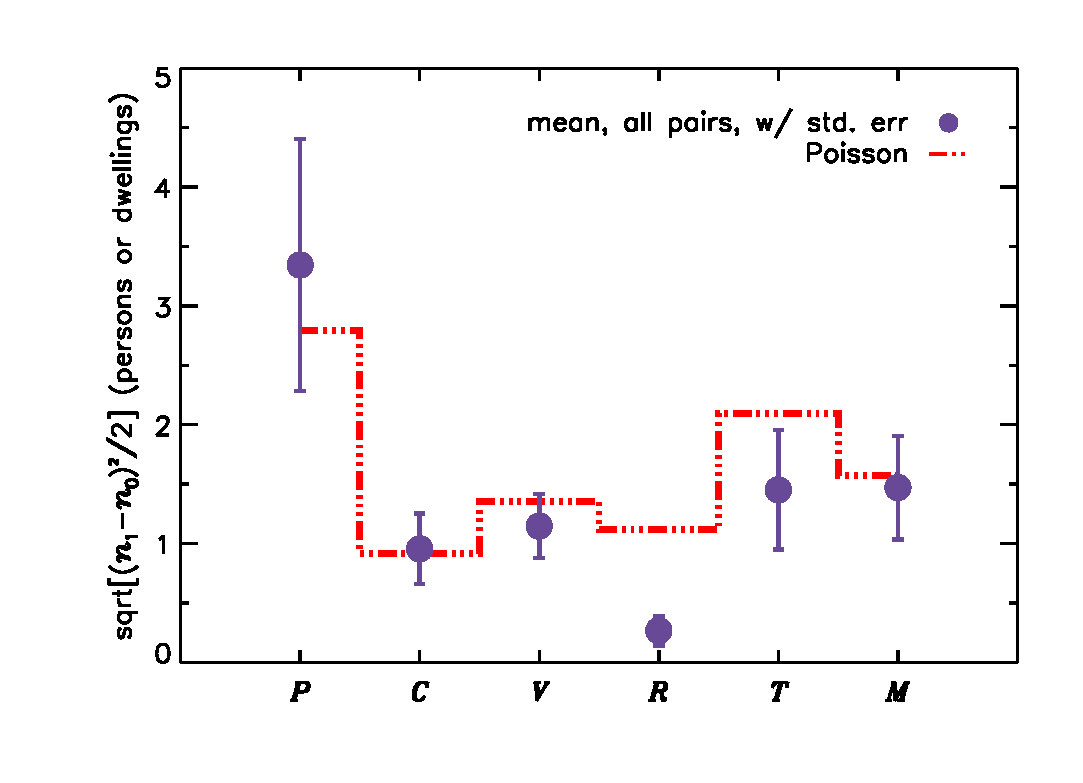
\includegraphics[width=\linewidth]{catDupeChar}
\caption{Duplicate tract (top) and category (bottom) count comparisons. Orange 
		points at top exclude tract 1901.00, which is a significant outlier.}
\label{fig:dupeChar}
\end{figure}

\subsubsection{Monte Carlo Estimations of Unsheltered Probability Densities}
\label{sec:mc}

Our analysis accounts for two known sources of uncertainty: Poisson errors in the visual tallies and 
random deviations of the CVRTM weights from their quoted means. The former represents how a given 
tally might change if performed at a different (but comparable) time or by a different team. The latter 
represents how the mean occupancy of CVRTM structures in Hollywood might differ from the mean 
occupancy in the geography in which the weights were defined.

We model both uncertainties as Gaussian distributions with standard deviations of 
$\sqrt{n}$ and $\sigma$, \resp, where $n$ is the raw tally and $\sigma$ is the standard 
error on the respective mean CVRTM weight, $w$, quoted by LAHSA. As such, the $i$-th estimate 
of the true number, $N$, of people in the $j$-th unsheltered class in any tract is:
\begin{multline}\label{eq:monte}
	N_{i,j} = \left[n_{j} + \mathcal{G}_{i}(0,\sqrt{n_{j}})\right]\times\max[\mathcal{G}_{i}(w_{j}, \sigma_{j}),1],
\end{multline}
where $\mathcal{G}(\mu,\Sigma)$ is a Gaussian random number with mean $\mu$ and standard deviation 
$\Sigma$. If more than one team counted a given tract, $n$ is replaced by the average of their tallies 
and the attendant counting error is divided by the square root of the number of teams.

The final output probability distribution functions (PDFs) are based on 10,000 realizations of 
Equation \ref{eq:monte}. For the Adult, and TAY, classes all weights are fixed to unity, such that 
$(w,\sigma)\equiv(1,0)$ for all trials and uncertainties reflect only counting errors. One potential 
family and one potential unaccompanied minor were reported, but not confirmed. We therefore
set those entires to zero, though still infer upper-limits.

We place a floor on the CVRTM mean occupancies at 1 person per dwelling; i.e., we assume that the average
person does not own more than one tent. This is not to say no one may own more than one tent, just that
such a statement is never representative. This choice induces a mild asymmetry in our global PDFs but
does not significantly affect inferences.
%letting the mean occupancies reach 0 moves the baseline result down by 40 ppl over all of grtr Hwood.
%it's 0.4 sigma or in the IQR.

\begin{figure*}[t]
	\centering
	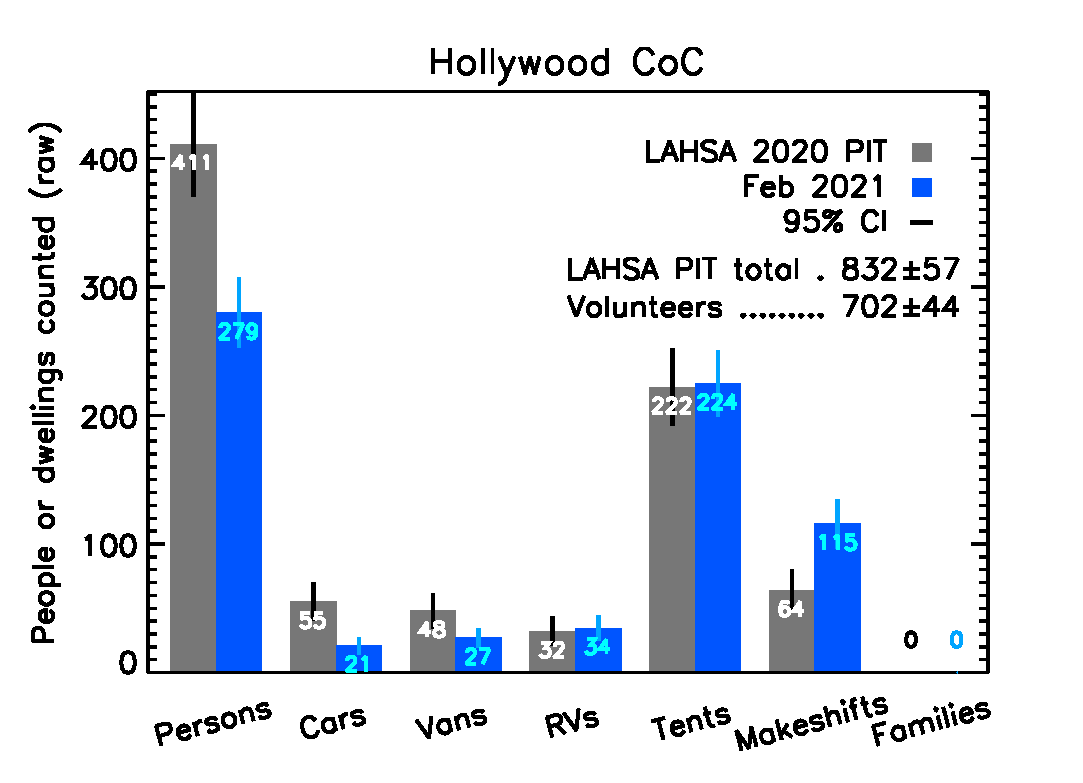
\includegraphics[width = 0.47\textwidth, trim = 1cm 0cm 0cm 0cm]{Hwood2021Bars}
	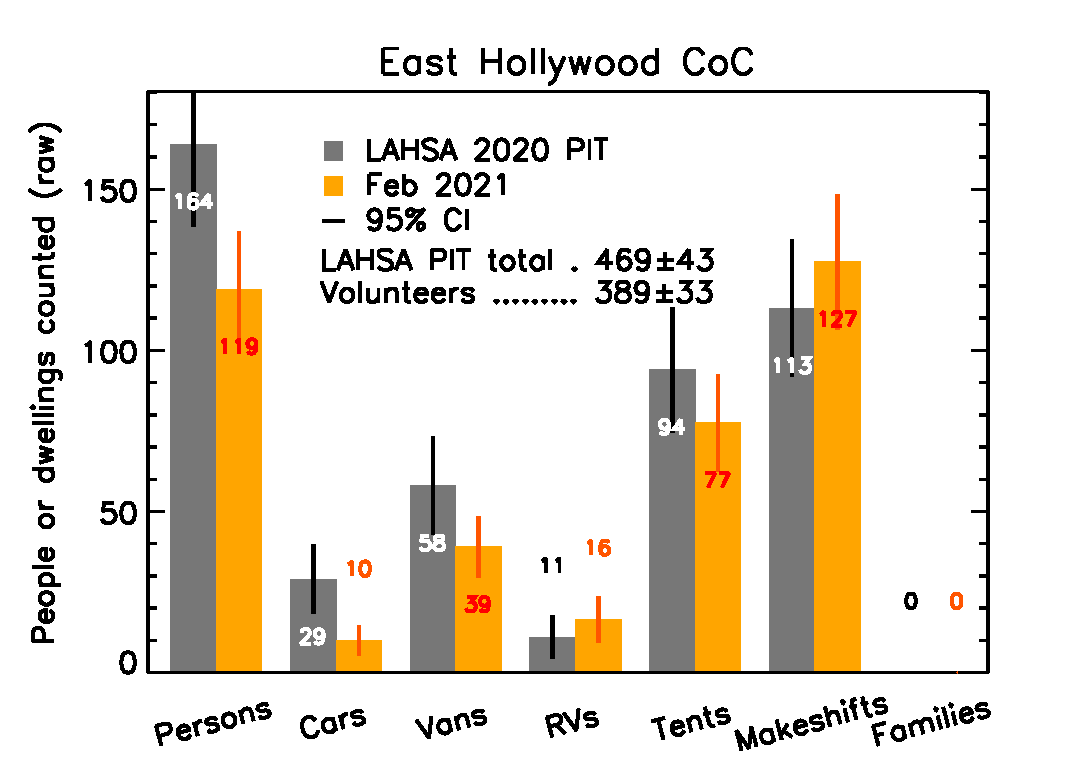
\includegraphics[width = 0.47\textwidth, trim = 0cm 0cm 1cm 0cm]{Eho2021Bars}
	\caption{Raw tallies of unsheltered persons and dwellings in Hollywood and East Hollywood
			(left/right) from the 2020 and 2021 PIT counts (grey/colors). Persons, cars, 
			and vans fell in both communities while RVs and tents stayed statistically flat. 
			Makeshift structures are the only category to show a potential common increase. 
			Overall, we identified 208 fewer people and dwellings compared to 2020,
			with similar 16\% decreases assessed by almost entirely independent teams
			in both communities. ``Persons'' are TAY+Adults.}
	\label{fig:rawCounts}
\end{figure*}

\begin{figure*}[t]
	\centering
	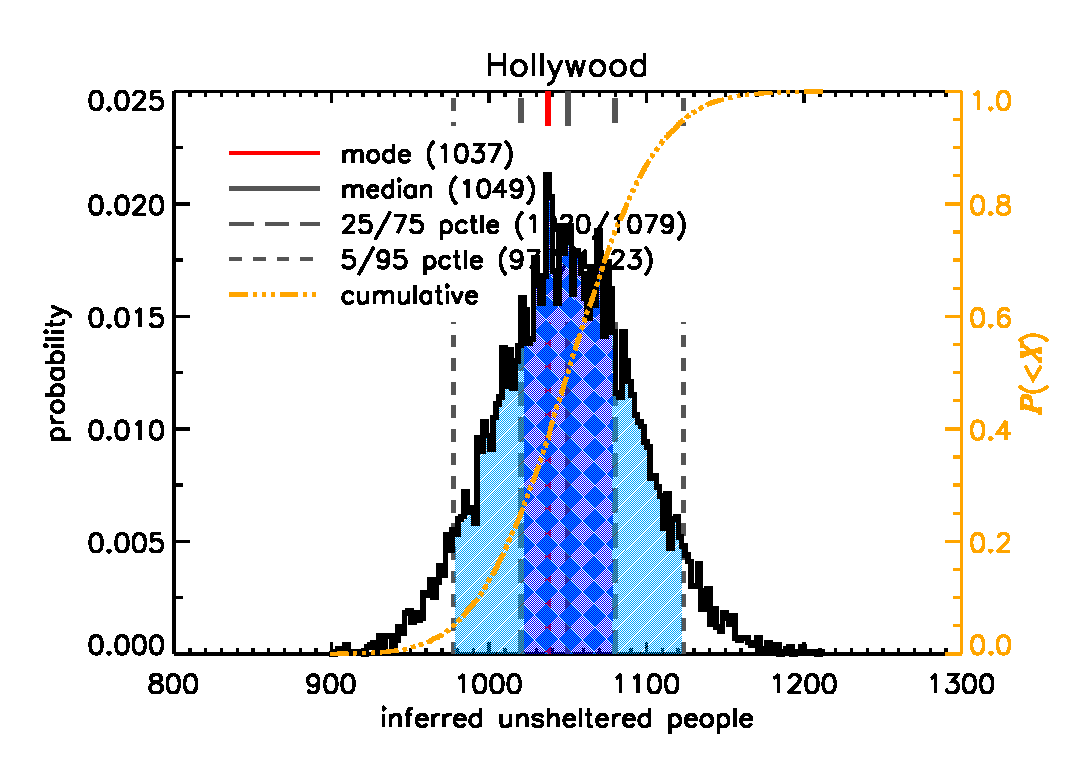
\includegraphics[width =0.47\linewidth]{hWood/HollywoodDist}
	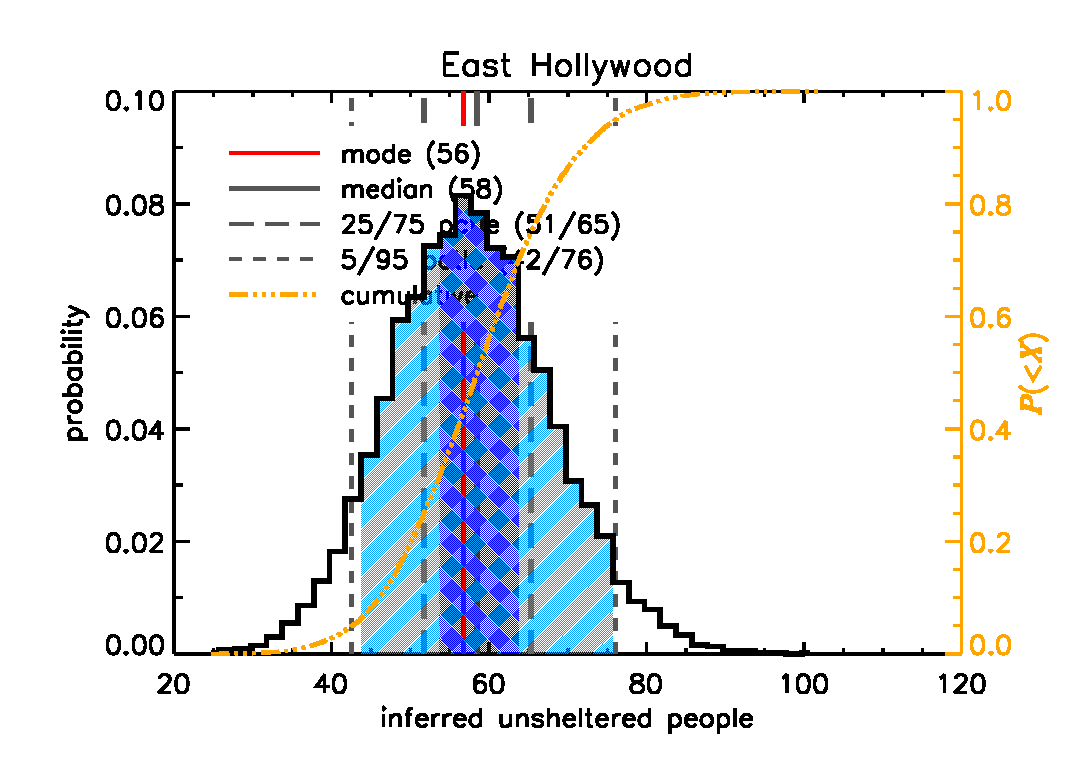
\includegraphics[width =0.47\linewidth]{eHo/EastHollywoodDist}
	\caption{}
\end{figure*}

\subsubsection{Null Entries}
\label{sec:nulls}

Some tracts were observed to have unsheltered populations near zero, at least in specific person or 
dwelling categories. These tallies are consistent with a range of non-zero values for the true population 
due to shot noise. As such, the Monte Carlo PDF reconstruction allows them to take non-zero values 
based on an assumed background rate. 

Ideally, that rate would be based on category variations in similar tracts defined by some independent 
criteria. Sufficient data from, e.g., the US Census may enable such an exercise, but it is beyond the scope of 
this analysis. Instead, we adopt a noise floor based on the counts expected if all elements of a given category
were evenly distributed across all tracts. Hence:
\begin{equation}
	\sigma_{j,\,\rm min}^{2} = \frac{1}{39}\sum_{\rm tracts}n_{j},
\end{equation}
where $\sigma_{j}$ and $n_{j}$ are defined as in Equation \ref{eq:monte}.

{\bfr tweak; not quite so-defined}

This method works for any category, $j$, for which there is at least one individual/dwelling observed in any 
tract. However, for categories for which this is not the case---unaccompanied minors and families, in the
case of Hollywood---we set $\sigma_{j, \rm min}$ to the lowest non-zero value of the other categories
(corresponding to TAY). The adopted backgrounds are: 
\begin{equation}
	\sigma_{j,\, \rm min}=\{3.2, 0.4, 0.4, 0.9, 1.3, 1.1, 2.8, 2.5, 0.4\}
\end{equation}
adults, TAY, unaccompanied minors, cars, vans, RVs, tents, makeshifts, and families per tract.

Such a treatment is somewhat arbitrary, but, since it is symmetric, and therefore unbiased, 
serves mainly to set the upper limits of intrinsically low-frequency categories (TAY, minors, families).

\subsection{Duplicate Counts}
\label{sec:dupes}

Each volunteer tract in both communities (30) were assigned to at least two independent counting teams.
Four tracts additionally received a third pass. Pass 1 was organized numerically by tract number.
Pass 2 paired high projected population tracts with a nearby tract. Pass 3 was the same as Pass 1 with 
tract pairings presented in reverse order (such that, if 2 teams were deployed simultaneously, they would
likely start in different tracts). 

Results for one of the two teams assigned to tract 1925.20 could not be interpreted, making it the only
volunteer tract with one population estimate.

Figure \ref{fig:dupeChar} shows the intercounter comparisons of raw counts (people+dwellings)
at the tract and category levels. Average offsets are close to Poisson expectations in all cases 
except for the highest occupancy tracts, where they are inflated by an outlier (see below).
Explicitly, $\langle\sqrt{(n_{1}-n_{2})^{2}/(n_{1} + n_{2})}\rangle=1.4$, where
$n$ are the total raw counts of dwellings and people in a given tract from one of the counting
teams. Given their salience, agreement in counting RVs is also significantly better than random 
errors would suggest.

The outlier is tract 1901.00, whose repeat measurements differ by $6.6\sigma$. There, 
one team counted $\{P,C,V,R,T,M\}=\{23,1,1,1,6,2\}$ while the other counted $\{77,15,10,1,6,6\}$. 
Abramson re-counted this tract on-foot 14 hours after the PIT tally, obtaining $\{36, 4, 6, 0, 8, 2\}$.
In total, this tally ($56\pm7$) is within 1.9$\sigma$ of the mean of the two volunteer teams ($75\pm6$). 
As such, we treat the PIT entries identically to the rest.  As illustrated in Figure \ref{fig:dupeChar}, top,
the mean intercounter variance drops (to $1.3\,\sigma$) if this tract is excluded.

%1901.00 inter-counter difference is 4.7 sigma (sqrt(delta) / root(n1 + n2) / root(2))

%\begin{itemize}
%%	\item All vol tracts counted at least twice;
%%	\item 4 tracts counted 3x;
%%	\item One recount DQed for quality flag (1925.20);
%%	\item Dupe statistics look pretty good. Mean abs discrepancy is consistent
%%		with zero given standard error on mean except for TAY (2.7 sigma) and RVs (3.8).
%%		Normalized differences ($|n_{1}-n_{2}|/\sqrt{n_{1}+n_{2}}$) are a little higher
%%		than $1\sigma$ ($CVRTM=[1.7, 1.1, -, 1.6, 1.4, 0.6, 1.2, 1.6, -]\sigma$), suggesting 
%%		a little more than poisson counting uncertainty, but LEA cross-checked the one
%%		highly discrepant ($\sim$8$\sigma$) tract, 1901.00, and found raw counts consistent
%%		with the average of the two nighttime datasets ($\sim$9:00 AM 26 Feb). 
%	\item Above holds true for 1912.01, which is in Hwood and also a SELAH recount tract. LEA
%		counted 51 totoal ppl/dwellings 12:30 P on 27 Feb vs 51 by vols night of count.
%\end{itemize}

No team counted tracts in both Hollywood and East Hollywood, making the volunteer tract datasets
totally independent in those communities. Once the professional-counted tracts are included, cross-talk
comes only from one tract in East Hollywood counted by a team that surveyed five tracts in Hollywood. 
We discuss comparisons between volunteer and professionally counted tracts in both communities 
in Section \ref{sec:comp}.





\begin{table*}[t!]
\centering
\caption{Greater Hollywood 2021 PIT Unsheltered Data and Population Estimates}
%\resizebox{\linewidth}{!}{%
\begin{tabular}{lccccc}
\toprule
 & $C$ & $V$ & $R$ & $T$ & $M$ \\ \cmidrule{1-6}
{\bf SPA4/CD13} & $1.51\pm0.25$ & $1.77\pm0.42$ & $1.42\pm0.28$ & $1.48\pm0.11$ & $1.68\pm0.31$ \\
2021 $T$ & -- & -- & -- & $1.39\pm0.14$ & --\\
2021 $T$ w/ unocc & -- & -- & --& $1.51\pm0.24$ & --\\
%2021 $T$ & $1.51\pm0.25$ & $1.77\pm0.42$ & $1.42\pm0.28$ & $1.39\pm0.14$ & $1.68\pm0.31$\\
%2021 $T$ w/ modeled unocc & $1.51\pm0.25$ & $1.77\pm0.42$ & $1.42\pm0.28$ & $1.51\pm0.24$ & $1.68\pm0.31$\\
SPA4 & $1.38\pm0.11$ & $1.68\pm0.22$ & $1.32\pm0.15$ & $1.45\pm0.06$ & $1.64\pm0.16$\\
\bottomrule
\end{tabular}
%}
\caption*{CVRTM weights tested. Dashes denote identical values to the entry above. Bold denotes 
baseline scenario incorporating the 
\href{https://www.lahsa.org/documents?id=4635-usc-2018-2020-multipliers-and-estimates-overview}
{2020 SPA4/CD13 CVRTM weights} underpinning the latest official Hollywood and East Hollywood 
\href{https://www.lahsa.org/documents?id=4686-2020-greater-los-angeles-city-community-homelessness-report-service-planning-area-4.pdf}{Community Summaries}.}
\label{tbl:weights}
\end{table*}

\begin{figure*}[t]
	\centering
	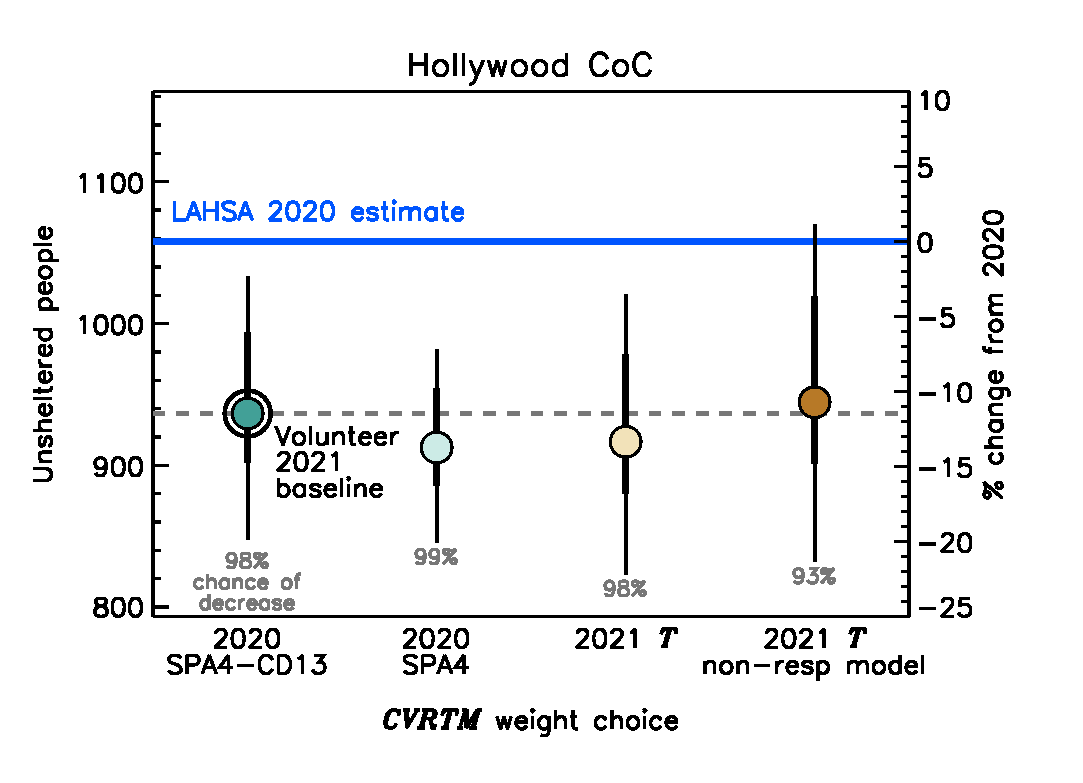
\includegraphics[width = 0.48\textwidth, trim = 0cm 0.5cm 0cm 0cm]{hwoodFinal}
	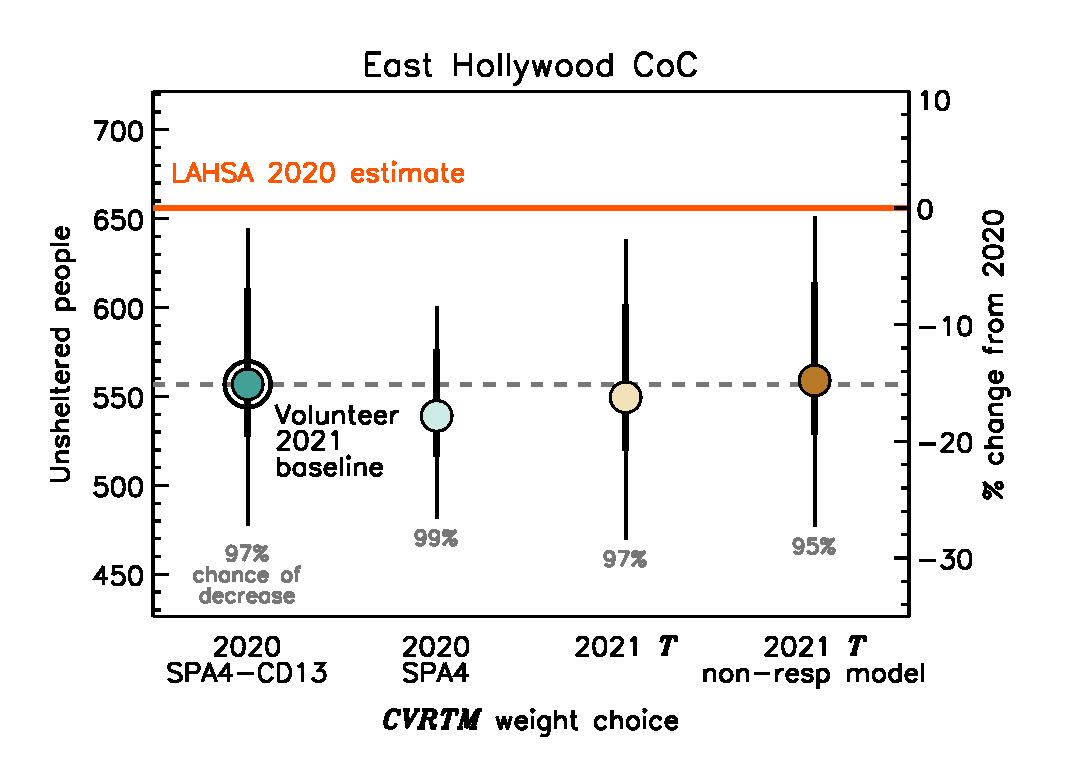
\includegraphics[width = 0.48\textwidth, trim = 0cm 0.5cm 0cm 0cm]{ehoFinal}	
	\caption{Unsheltered populations in Hollywood (left) and East Hollywood (right) 
			as functions of CVRTM weights. The baseline estimate uses the same weights as the 
			2020 LAHSA Community Summaries. Using SPA4 weights or replacing the tent 
			weight, $T$, with results from a survey conducted in Hollywood yields consistent
			results. All imply at least a 93\% chance that unsheltered homelessness has fallen
			by some amount, with likely declines of $12\%\pm9\%$ and $15\%\pm12\%$
			in Hollywood and East Hollywood, \resp.}
	\label{fig:wtComp}
\end{figure*}

%{\bfr PRO TRACT RAW COUNT SHARE 2020: 44\% (23 tracts)
%
%PRO TRACT RAW COUNT SHARE 2021: 43\% (all tracts)}
%
%{\bfr Barely consistent if all of last year's vans and cars are still here. 95\% confidence limit $996\pm69$ can reach 1065 (v 1058) 
%in Hollywood, $598\pm 59= 657$ vs.\ 656 last yr in E.~Hollywood. BOTH AT 2020 SPA4 WEIGHTS!}


\section{Results}
\label{sec:results}

This section presents community level estimates for the number of unsheltered people living in
Hollywood and East Hollywood as of 25 February 2021. We start with summaries of each community 
in Sections \ref{sec:hWood} and \ref{sec:eHo} before discussing how those inferences compare to 
the official 2020 LAHSA data in Section \ref{sec:comp}. 

%Section \ref{sec:discussion} describes how 
%varying elements of Section \ref{sec:mc}'s analysis modulates these results.

\subsection{Hollywood}
\label{sec:hWood}

, from which we also draw 2020's person and CVRTM raw tallies. Those inferences yield 
$936\pm92$ and $556\pm83$ people experiencing unsheltered homelessness, \resp\ (90\% CI). Modifying the weights
to their 2020 \href{https://www.lahsa.org/documents?id=4693-2020-greater-los-angeles-homeless-count-cvrtm-conversion-factors}
{SPA4-wide} values or using data from in-person surveys of tent-dwellers in Hollywood has no
significant effect.\footnote{Those inferences yield $912\pm68$ and $944\pm118$ people
in Hollywood, and $539\pm59$ and $559\pm87$ in E.~Hollywood, \resp.} 
All estimates suggest at least a 93\% chance of a decline compared to the 2020 PIT count.
 % (Figure \ref{fig:wtComp})

Nevertheless, the CVRTM weights are systematic uncertainties: if the average tent or makeshift structure holds
more people today compared to last year, then the inferred population decrease may be artificial. Given the drop in 
unweighted counts, however, those dwellings' {\it average} occupancies must have risen to 2.2 and 2.6 people 
from 1.5 and 1.7 people, \resp, to erase the decline. Such $\sim$50\% increases in the mean seem unlikely given 
known COVID-related tent distribution efforts---which push in the opposite direction---and a 28 Feb.\ tent 
survey yielding a weight consistent with 2020's value.\footnote{The $T$ and $M$ weights are the largest 
potential error sources in this analysis due to the high proportion of people living in tents and makeshift structures. 
While the full 2021 PIT area has not been assessed, SELAH outreach teams surveyed 47 tents (38 responses) in 
Hollywood on 28 Feb., yielding a mean occupancy of $T=1.39\pm0.14$ people per tent ($T=1.50\pm0.22$ when 
non-responses are modeled). Although $M$ was not estimated, that $T$ value is consistent with the official 2020 
weight of $T=1.48\pm0.11$. We encourage more robust efforts to update the CVRTM weights.} 
%the occupancy increases needed to erase our estimated changes are
%substantial. 

Multiple cross-checks suggest that the raw counts from our 2021 PIT enumeration are accurate:
\begin{enumerate}
%	\setlength{\itemsep}{-1ex}
	\item Comparisons of the count's 37 duplicate tract measurements suggest per-tract and per-category
		counting uncertainties are consistent with the random errors built into the analysis.
%		\begin{itemize}
%			\item Tract 1901.00---the only outlier in the above comparisons---was independently recounted 
%				14 hours after the PIT count with results consistent with the average of the volunteer teams' 
%				results.
%			\item Tract 1912.01---largest increase---was independently recounted on 27 Feb.\ circa 
%				12:00 PM with results similarly consistent with the PIT teams' assessments.
%			\item Tract 1927.00---largest decrease---was independently recounted on 4 March at 
%				8:30 AM with results lower than the PIT's assessment. This especially dense tract was originally 
%				surveyed on foot by outreach professionals, however, with the recount was performed by a car-based
%				volunteer. The cross-check therefore suggests only that the PIT data are not biased in ways that
%				would induce an artificial year-on-dear decline.				
%		\end{itemize}
	\item External data from \href{https://hollywoodpartnership.com/}{\it The Hollywood Partnership} 
		from 19 Feb.\ are consistent with our PIT count in a common tract (1902.02) and an independent 
		recount of that entire geography performed 28 Feb.% also show a decline from past values and 
	\item Trends hold in tracts counted by volunteers and professionals in Hollywood and East Hollywood.
	% (reduced individuals, flat
%		or marginally higher dwelling counts).
%	\item Tracts monitored by \selah\ since May 2020 show similar declines to that implied by our data. 
%		One of these tracts is 1912.01 in East Hollywood, whose 27 Feb.\ \selah\ estimate  agrees with our 
%		PIT value.% in unsheltered homelessness.
	\item A 27 Feb.\ recount of tract 1912.01 in East Hollywood conducted as as part of a
		\href{https://selahnch.org}{SELAH} monitoring campaign agrees with our PIT value.% in unsheltered homelessness.
\end{enumerate}

%		   P	C     V	    R	 T     M
%1901.00 -- 50    8    5.5   1     6      4 -- 2021, raw
%1901.00 -- 36    4     6     0     8      2 -- 26 Feb ABRAMSON 9.00 AM
%
%1927.00 -- 48    1      5     0    53    70 -- 2020, raw
%1927.00 -- 20    0     0     7     6     54 -- 2021, raw
%1927.00 -- 15     0     9     5    14    21 -- 4 Mar 2021 ABRAMSON 8.45 AM
%
%1912.01 --  18.5  0.5  3.5  1.5  5.5  12 -- 2021, raw
%1912.01 --  21     0      4     1     8      6  -- 27 Feb ABRAMSON 12.15 PM
%
%1902.02 -- 9      --     --     --     8   5.5 -- 2021, raw
%1902.02 -- 9      --     --     --    17    --  -- BID 2/19

% 1907.00 is also interesting in that total population stayed nearly the same but identified
% individuals and dwellings basically swapped: IND 73->38; CVRTM 31->70. This has a big impact
% on people's perceptions, and it's in a very high-traffic part of the community.

%The pro/vol trends are consistent everywhere except tract 1927.00, 
%			where pro counts dropped significantly more for both individuals and dwellings (esp.\ 
%			tents). 1927.00 comprises 22\% of total counts in East Hollywood. Unsheltered 
%			homelessness in that CoC was flat or rose slightly outside of that tract.}
%{\bfr 1927.00 is the tract with the PATH Madison PSH. Phase II opened in Jan 2020---leasing began May 
%2020---and is 120 units, some of which were filled from nearby folks but I dunno how many. LEA recounted 
%this tract 4 March at $\sim$9:00 AM and found 94 total population vs.\ pro's 129. Only place where
%LEA counted more objects was vans. Adding that to the pro total adds 16 people (9 vans).

{\bfr Up to the number of vehicle dwellers in safe parking locations,} the above suggests that our results 
are both quantitatively and qualitatively reliable.\\

\subsection{East Hollywood}
\label{sec:eHo}

\begin{figure}[]
	\centering
	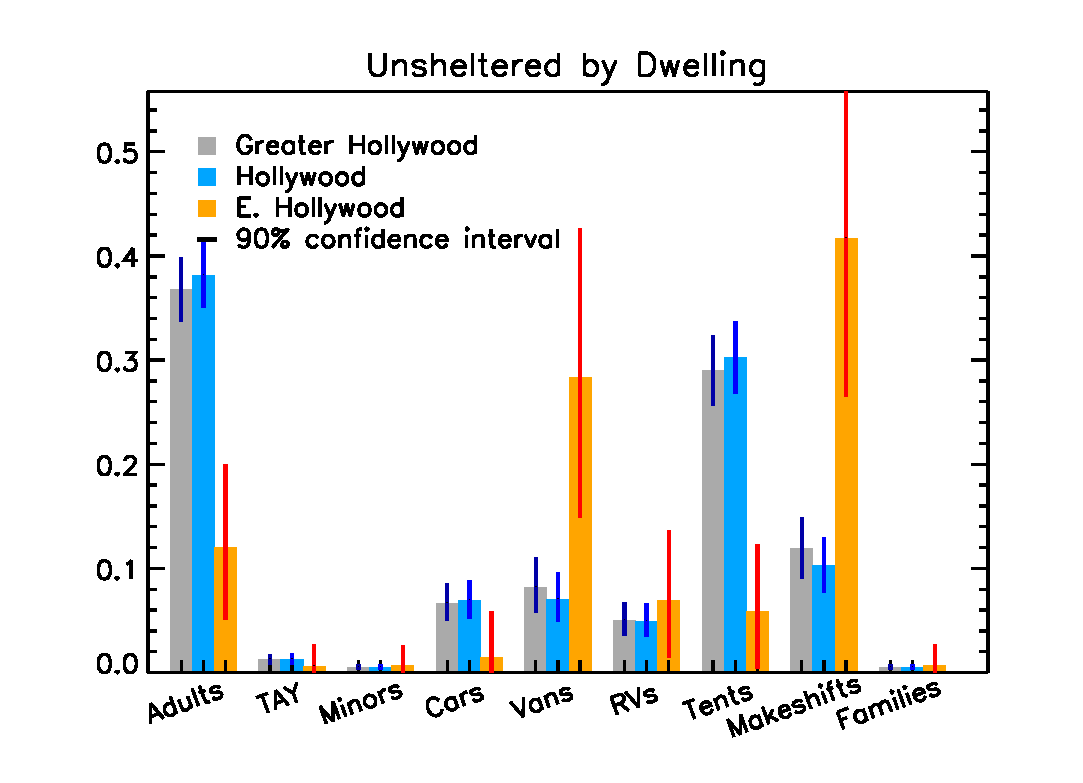
\includegraphics[width =\linewidth]{allTracts/allBreakdownBar}
	\caption{}
\end{figure}

\subsection{Comparison to 2020}
\label{sec:comp}

\begin{figure*}[]
	\centering
	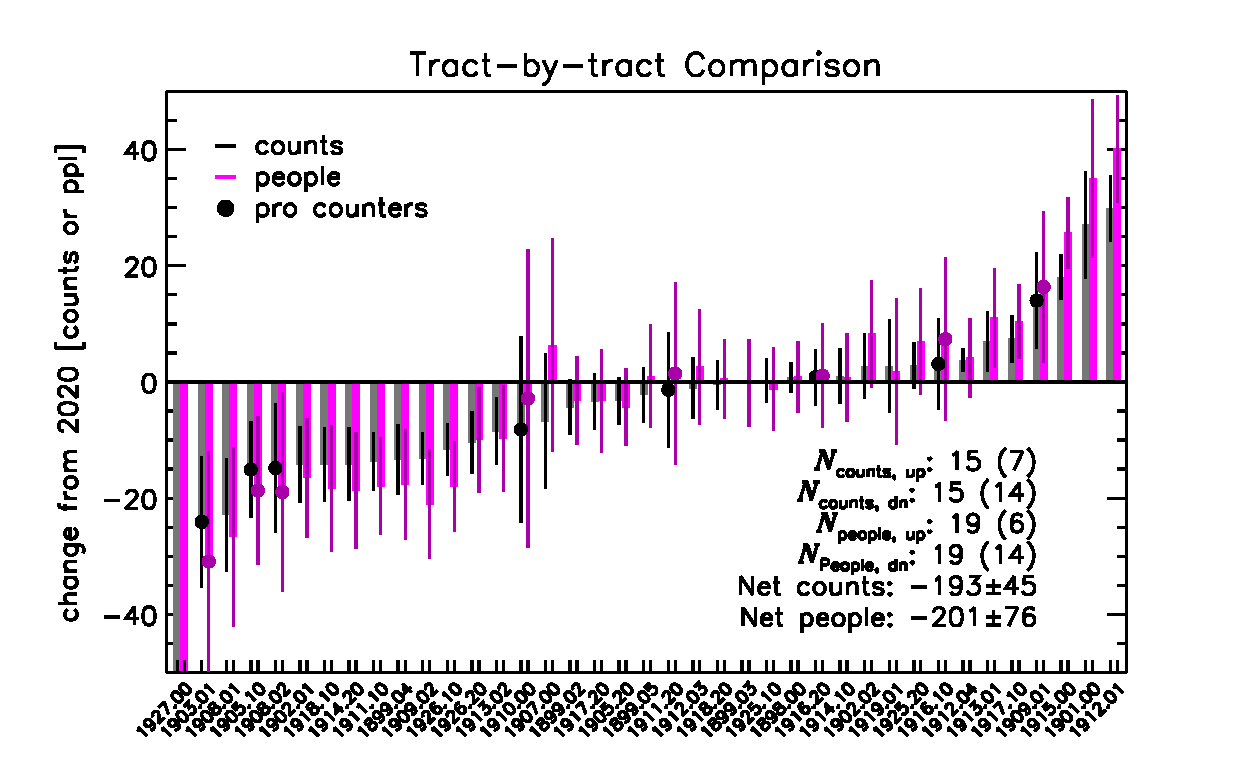
\includegraphics[width = \linewidth, trim = 0cm 0cm 0cm 0cm]{tractsYrYr}
	\caption{}
	\label{fig:tractYrYr}
\end{figure*}


\subsubsection{CVRTM Effects}
\label{sec:CVRTM}



\begin{figure}[]
	\centering
	\includegraphics[width =\linewidth]{volProfComp}
	\caption{}
\end{figure}


\begin{table*}[t!]
\caption{Greater Hollywood 2021 PIT Unsheltered Data and Population Estimates}
\resizebox{\linewidth}{!}{%
\begin{tabular}{lcccccccccc}
\toprule
 & Adult & TAY & Car & Van & RV & Tent & Makeshift & {\bf 2021 Total} & {\bf 2020 Total} & {\bf Difference} \\ \cmidrule{1-11}
{\bf Hollywood} \\ %\cmidrule{1-1}
Counts & 277 & 2 & 21 & 27 & 34 & 224 & 115 & {\bf 702} & {\bf 831} & $\bf -15\%$ \\
Inhabitants & 277 (27) & 2 (5) & 32 (11) & 49 (13) & 50 (14) & 332 (29) & 195 (24) & {\bf 937 (93)} & {\bf 1058} & $\bf -11\%\,(9\%)$\\% (76)
Category share & 30\% (3\%) & 0\% (0\%) & 3\% (1\%) & 5\% (1\%) & 5\% (1\%) & 35\% (3\%) & 21\% (3\%) & -- & -- & -- \\ \cmidrule{1-11}
{\bf East Hollywood} \\ %\cmidrule{1-1}
Counts & 114 & 4 & 10 & 39 & 16 & 77 & 127 & {\bf 389} & {\bf 469} & $\bf -17\%$ \\
Inhabitants & 114 (19) & 4 (4) & 15 (8) & 70 (15) & 24 (9) & 115 (19) & 216 (23) & {\bf 557 (83)} & {\bf 656} & $\bf -15\%\,(12\%)$\\% (60)
Category share & 20\% (3\%) & 1\% (1\%) & 3\% (1\%) & 13\% (3\%) & 4\% (2\%) & 20\% (3\%) & 39\% (4\%) & -- & -- &--
\\ \bottomrule
\end{tabular}
}
\caption*{Parentheses denote 90\% uncertainties(binomial in the case of the categories). 
Uncertainties larger than estimates imply that only upper limits are available. No unaccompanied 
minors or families were observed.}
\label{tbl:summary}
\end{table*}

Less easily handled are potential biases in the CVRTM demographic weights our \Count\ adopts.
Typically, specialized teams perform detailed interviews of people experiencing homelessness to update 
these weights in various geographic contexts. However, the cancellation of the official PIT count means
that this will not occur in 2021. As such, we are forced to rely on year-old estimates.


\subsubsection{Using External Data}
\label{sec:bidData}

The Hollywood Partnership---one of Hollywood's Business Improvement Districts (BIDs)---has performed
weekly visual scans of its footprint since spring 2019. These inspections tally unsheltered people and 
tents separately. As such, they can be used to bound the possible evolution of the CVRTM tent weight
between the official 2020 value and what it may be today.

{\bfr SECZ}

A lower-bound on the the weight can be derived by assuming that all of the tents captured by the BID's 
censuses were empty and all of their inhabitants visible. The weight would the be just the number of
people on the number of tents. If any of the tents were not empty, the true weight would be higher than
the inferred weight. Ergo, the BID/SECZ derived tent weight may reflect a {\it conservative} estimate 
which, when applied to the entire footprint, would produce something like a lower-bound on the 
tent contribution to the 2021 \Count.

{\bfr We'll use the BID counts outside the SEZ and find (tents+people)/tents for the past year. We'll
fit it and get a range of values for the night of the count. It's typically higher than 1.45 (thru last July,
at least), so we can just find the decline and peg it to 1.45.}

{\bfr Plot the trend; discuss it in terms of the 2020 value; see what it does; talk about why we don't
think most of the folks on foot in the SECZ are interlopers.}

\section{Discussion}
\label{sec:discussion}

\subsubsection{Nulling the 2021 Result}
\label{sec:nullOut}

\begin{figure}[]
	\centering
	\includegraphics[width =\linewidth]{tract1907comp}
	\caption{}
\end{figure}

PRK effects.

ABH effects.

PSH effects.

{\bfr 1907.00 people and tents switched. Total unsheltered $\sim$constant but visual perceptions
in this most-highly trafficked tract will make it *feel* like homelessness has increased by a lot.}

SPLA.

Edges.

Deaths.

\section{Summary}
\label{sec:summary}

\section*{}

{\bfr Acknowledge Kelson}

\appendix

\section{Example Documents}

\begin{figure*}
	\centering
	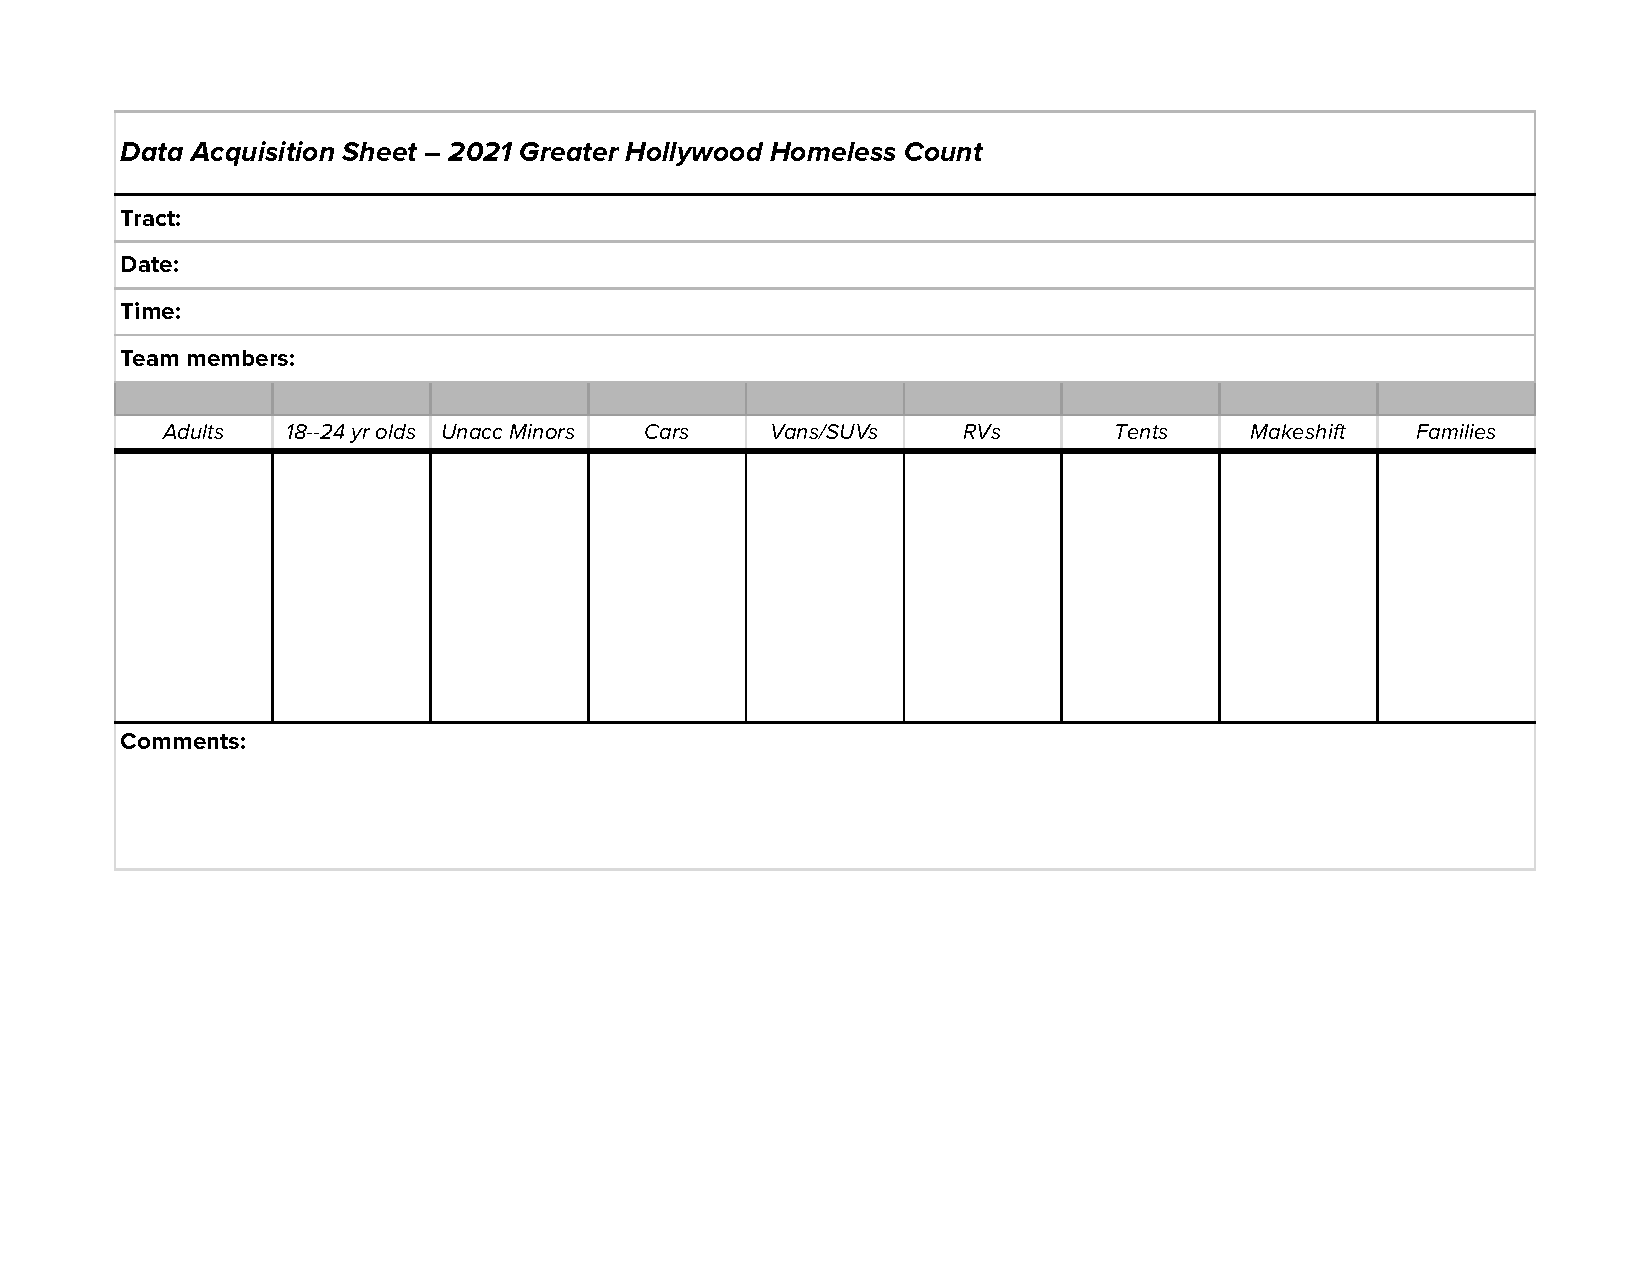
\includegraphics[width =\linewidth]{Hollywood2021CountDataSheet}
	\caption{Counter tally-sheet}
\end{figure*}

\begin{figure*}
	\centering
	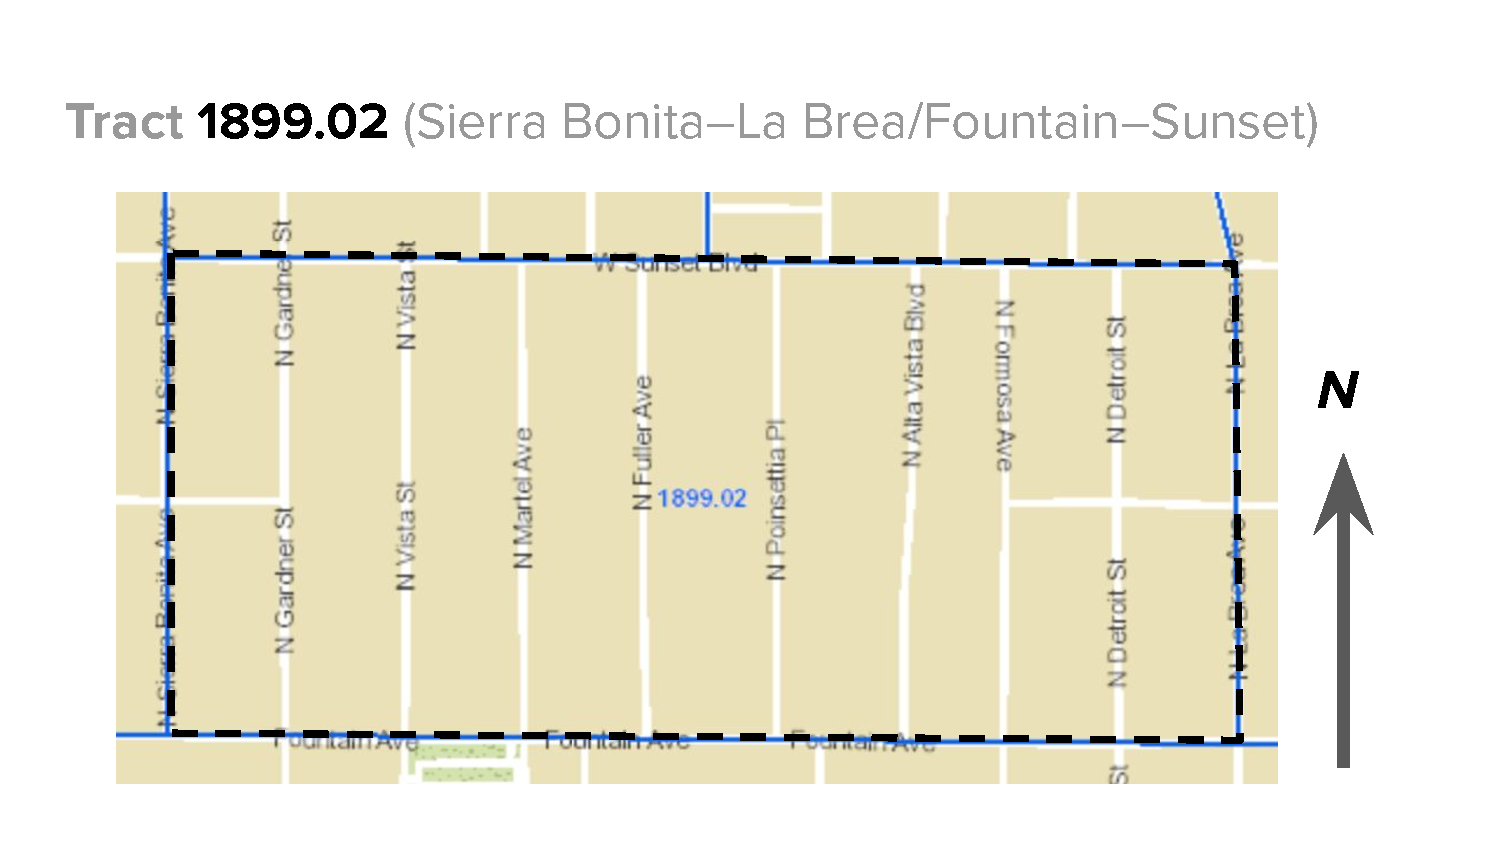
\includegraphics[width =\linewidth]{tractMap}
	\caption{Example Hollywood tract map.}
\end{figure*}

\begin{figure*}
	\centering
	\includegraphics[width =0.7\linewidth]{primerFront}
	\caption{Count primer {\bfr SCRUB EK'S NUMBER!}}
\end{figure*}

\section{Full Tract-level Results}


\begin{table*}[]
\caption{Tract 1898.00 Unsheltered Data}
\resizebox{\linewidth}{!}{%
\begin{tabular}{lcccccccccc}
\toprule
 & Adult & TAY & Unacc Minor & Car & Van & RV & Tent & Makeshift & Family & {\bf Total} \\ \cmidrule{1-11}
Counts & 3 & 0 & 0 & 0 & 0 & 0 & 1 & 1 & 0 & {\bf 5} \\
Inhabitants & 3 (3) & 0 (1) & 0 (1) & 1 (2) & 1 (2) & 1 (2) & 2 (2) & 2 (2) & 0 (1) & {\bf 9 (6)} \\
Category share & 0.31 (0.29) & 0.03 (0.10) & 0.03 (0.10) & 0.09 (0.18) & 0.10 (0.19) & 0.07 (0.16) & 0.16 (0.23) & 0.18 (0.24) & 0.03 (0.10) & - 
\\ \bottomrule
\end{tabular}
}
\caption*{Quantities in parentheses denote 95\% uncertainties (binomial in the case of the categories). Uncertainties larger than estimates imply that only upper limits can be stated confidently.}
\label{tbl:}
\end{table*}

\end{document}  